\documentclass[a4paper,12pt]{article}

\usepackage{préambule}

\title{Sondage : Pointure}
\author{Mr Golfouse}
\date{}

\renewcommand{\arraystretch}{1.2}

\begin{document}

\maketitle

Notre sondage porte sur la pointure des élèves, un sujet très important !

\subsection*{Résultats}

Nous avons interrogé 25 élèves au total :

\begin{center}
	\begin{tabular}{|l|c|c|c|c|c|c|c|c|c|}
		\hline
		Pointure  & $35$     & $36$     & $37$     & $38$     & $39$     & $40$    & $41$               & $42$     & $43$
		\\ \hline
		Effectif  & $2$      & $4$      & $4$      & $2$      & $4$      & $5$     & $0$                & $1$      & $3$
		\\ \hline
		Fréquence & $0{,}08$ & $0{,}16$ & $0{,}16$ & $0{,}08$ & $0{,}16$ & $0{,}2$ & \phantom{$0$}$0$\phantom{$0$} & $0{,}04$ & $0{,}12$
		\\ \hline
	\end{tabular}
\end{center}

\subsection*{Diagramme}

\begin{center}
	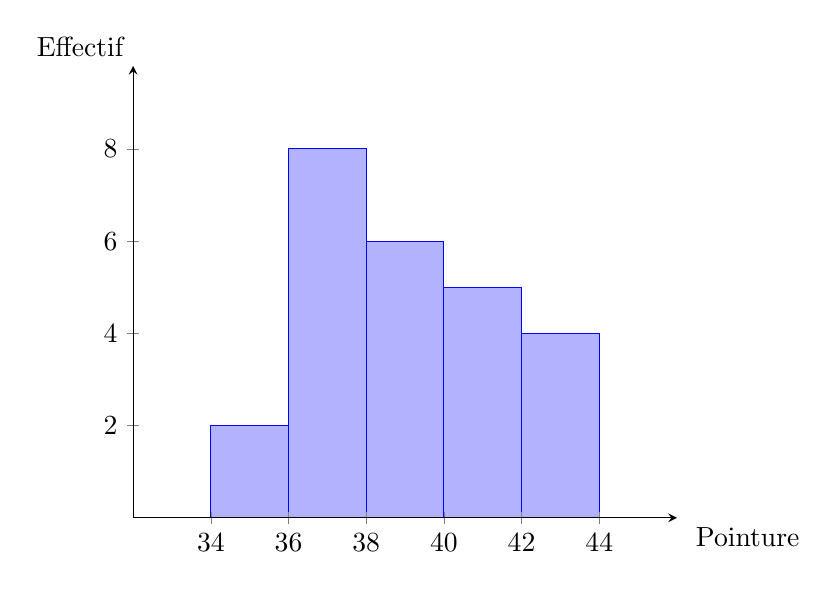
\begin{tikzpicture}
		\begin{axis}[
				width = 0.7\textwidth,
				xmin=32, xmax=46,
				ymin=0, ymax=9.8,
				axis lines=center,
				ylabel={Effectif},
				xlabel={\ Pointure},
				xlabel style={below right},
				ylabel style={above left},
				area style,
				xtick=data
			]
			\addplot+[ybar interval,mark=no] plot coordinates { (34,2) (36,8) (38,6) (40,5) (42,4) (44,0) };
		\end{axis}
	\end{tikzpicture}
\end{center}

\subsection*{Moyenne}

La moyenne des pointures était $38{,}6$.

\end{document}